\section{论文研究背景与意义}

\subsection{论文选题背景}

\subsubsection{实际应用背景}
随着我国法制制度建设的不断完善,居民法律意识也日渐增强,
对司法系统的依赖程度也越来越高,这就导致案件数量激增,
大量的刑事或民事案件流入司法系统,
这种情况对司法系统的办案效率提出了更高的要求。

据程金华\upcite{chenjinhua}等人的研究调查显示:
近年来,中国法院的诉讼案件量持续上升,
先后几任最高院院长在每年全国“两会”工作报告中,
都明确提到法院系统“案多人少”和法官工作负荷重的问题。
改革开放以来,中国法院的诉讼案件量一直在高速增长。
1993 年,全国法院刑事、民事、行政和执行案件
的立案总量为 460 多万件,到 2019 年增加到 2652
万余件,在不到30年的时间里,增加了4.75倍。
一起案件的审理需要司法工作人员在仔细阅读案情描述的基础上参考大量诸如法律条文、
涉案证据、历史案件等资料,并依托自身专业知识进行涉案证据的核实与整理,
最终给出涉案人员罪名裁定,刑期的判决,以及给出最终的法院观点。
不难看出,司法人员无论是在体能、工作压力,
还是在业务能力、办案效率等方面正面临着越来越严峻的挑战。

我国法律体系是成文法系,其法律以成文法的方式存在,
这也就意味着我们在进行定罪的时候,必须找到能够证明相关法条的证据。
证据在司法案件定罪和量刑中都起到了极其重要的作用,
目前我国法律文书中,大部分文书将同一个案件所涉及到的所有证据仅仅进行简单的罗列,
这一做法导致证据的论证性以及不同证据之间的关联性缺失。
因此,对司法案件中涉及到的证据进行合理的组织不仅能够提升定罪的推理逻辑性与完备性,
也使得判决结果更具可解释性\upcite{bibal2021legal}。

\subsubsection{学术界理论研究背景}


此前的工作提出了多个功能多样的法律辅助系统,
如给定案情描述搜索相关案件\upcite{chen2013text},
预测法律判决\upcite{ye2018interpretable}等。
尽管这方面的研究成果丰富多种,
但是依旧存在两个问题,
首先,当前最先进的 (SOTA) LJP 模型面临的技术问题之一是
它们未能定位能确定判断结果的关键信息\upcite{zhong2018legal,xu2020distinguish}。
其次,近年的研究忽略了来对刑事案件司法证据的研究。
司法证据的作用是论证用于定罪的若干子论点,
而证据说明是刑事判决书的重要组成部分。

近年来,一些论文也关注到了
司法决策模型没有定位到关键信息,
导致缺乏可解释性的问题。
但是这些论文,并没有从法律条文出发对案情描述关键信息的识别
进行针对性的预测和评估。
论文\upcite{chao2019interpretable}虽然通过关键信息进行下游任务预测,
但是没有给出对案情描述关键信息的预测结果进行量化评估。
论文\upcite{feng2022legal}虽然标注了一部分的案情描述关键信息位置,
并且给出了定位关键信息如何影响司法预测任务的结果,
但是这部分的关键信息标注并非在法条指导下的,
而是按照事件模式对案情描述进行的标注,
其标注内容无法与法律条文和司法论点相匹配,
可解释性和可扩展性都不足。

论文\upcite{teng2021argumentation}首次研究了司法证据相关的预测,
并构造了一个司法证据的数据集,
但其提出的是一种论证驱动的监督学习方法来计算证据对之间的距离,
并用于下一步的证据关联,
证据关联是根据相应的司法论点
将一组司法证据划分为几个不重叠的子集,
从而提高了论点可解释性和合法性,
但该任务是关联给定的已有证据,
缺乏对给定案情描述的直接证据预测。
据本工作调研所知,学术界关于法律领域的证据预测的研究非常有限。

% \subsubsection{项目研究背景}

\subsection{研究现状概述}
\subsubsection{司法智能化的研究现状}

司法智能化主要是指人工智能与司法的结合,
让人工智能技术能够辅助法律从业人员完成相应的工作。
如\cref{LJP}所示,
目前主要的研究方向有罪名预测、法条推荐、刑期预测、法院观点生成等
\upcite{feng2022legalSurvey,cui2022survey}。

\begin{figure}[h]
	\centering
	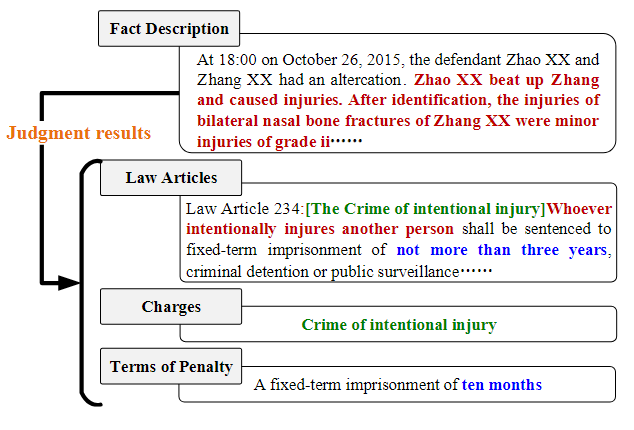
\includegraphics[width=0.6\linewidth]{LJP.png}
	\caption{司法智能化主要任务示例}
	\label{LJP}
\end{figure}

罪名预测指的是根据案件的事实描述来预测最终的判决罪名,
属于法律判决预测的子任务,在智能司法中起着重要的作用,
可以为法律人士提供方便的参考以提升工作效率,
也可以为不熟悉法律术语以及复杂判决流程的普通民众提供法律咨询工作。

大多数的罪名预测工作是以文本分类的方法去实现。
在早期,研究学者侧重于从事实描述等文本来提取有效的特征,
例如Lin等人\upcite{lin2012exploiting}通过人工设计罪名的相关规则来实现罪名预测,
但是这种方法需要耗费大量人力、精力去设计特征规则,
并且对于设计者的法律专业素养有着较高的要求,
无法推广到其他场景中。
因此,之后的学者开始使用发展迅速的深度神经网络来建模法律文档,
例如Luo\upcite{luo2017learning}采用基于注意力的神经网络,
对法律条文提取和罪名预测进行联合建模,
通过整合法律条文信息来实现更准确的罪名预测效果。
随后,Hu等人\upcite{hu2018few}考虑到司法领域中不同罪名间存在的数据不平衡问题,
一些不常见罪名涵盖的案件数量极少,
并且以往很多研究都是侧重于常见罪名的预测,
因此他们引入了10种额外的属性特征来辅助预测最终罪名。

而Liu等\upcite{liu2005classifying}通过一组固定的法条组合将多标签问题转换为多类别的分类问题,
之后Liu\upcite{liu2015predicting}首先通过支持向量机先进行法条的粗略分类,
获得一部分可能的罪名后再通过一些基于特征的重排序来确定最终的判决罪名。
Zhong等人\upcite{zhong2018legal}和Yang等人\upcite{yang2019legal}都是采取一个全局范围的思路,
模拟实际法官的行为,
综合考虑法律案件描述、适用法条、罪名预测、量刑预测等多个模块,
将几个模块串联起来共同学习训练,从而实现较为准确的量刑参考。

针对法院观点生成,
Jiang等人\upcite{ye2018interpretable}
针对这一需求提出一种在给定罪名条件下自动化生成判决文书的Seq2Seq模型。
另外,除了面向判案流程的研究以外,
法律领域的知识问答系统也是一个备受关注的课题。
这种问答系统可以为用户提供便捷的咨询服务。
Wu等人\upcite{wu2020biased}
提出了一种基于注意力和反事实的自然语言生成方法,
该方法使用注意编码器利用法条和案情描述作为输入来学习法条感知编码器,
从该编码器可以强调案情描述中的法条相关信息。
反事实解码器用于消除数据中的混淆偏差,
并通过结合协同预测模型生成。
Kim和Xu等人\upcite{kim2014legal}通过合并法律领域知识和文本细节特征完成对问题答案的检索。
Danilo等人\upcite{carvalho2015lexical}则通过融合信息抽取和知识问答提供了一套案情分析系统。

Xiao等人\upcite{xiao2021lawformer}
基于Longformer的预训练语言模型,
提出了中国法律长文件预训练语言模型,
称为Lawformer,用于中国法律长文档理解。
Lawformer在各种智能司法任务上进行了评估,
包括判断预测、类似案例检索、法律阅读理解和法律问答。
实验结果表明,
Lawformer可以在以长文档作为输入的任务上实现部分的改进。

\subsubsection{案情关键信息识别相关研究现状}

由于单篇案情描述文本长度过长,
通常能达到300-400字的篇幅,
所以,引导模型关注到案情描述中的关键信息,
而忽略掉一些影响较小的文本,
能够大幅提高与案情描述相关的智能司法任务的性能。
一部分的论文工作注意到了这一点,
从而有了对案情关键信息识别工作。

Jiang等人\upcite{chao2019interpretable}
通过从案情描述中提取出能决定罪名预测的文本片段
来增加罪名预测的可解释性。
这些语义片段是在罪名预测过程中提取的,
对预测结果具有决定性的影响。
因此,它们可以看作是罪名预测的解释,
提高了罪名预测的可解释性。
这篇工作认为从案情描述中抽取出的好的片段必须满足三个标准:
1)总长度应该很小; 
2)能够决定罪名; 
3)表达完整的语义。
但是这篇工作中语义片段的抽取完全靠文本的注意力机制,
并没有直接的监督数据。
如果存在一些情况,
法条文本和案情描述的语义上差别较大,
则无法进行抽取。

Feng等人\upcite{feng2022legal}
则进行了语义匹配标注。
他们利用从案情描述中提取事件信息的方法提取来解决LJP任务。
如\cref{event}所示,他们首先定义了一个层次事件结构,
并收集了一个新的带有事件注释的智能司法任务数据集。
之后,提出了一个模型,
该模型根据两种约束来联合学习智能司法任务和事件提取任务。
虽然该模型识别出并由于判断的案情事件信息具有一定的司法原理,
但是,事件的各项属性与法律条文中强调的判案维度并没有直接联系。
所以,使用这一些信息来理解案情信息,
是不全面且缺少司法可解释性的。

\begin{figure}[h]
	\centering
	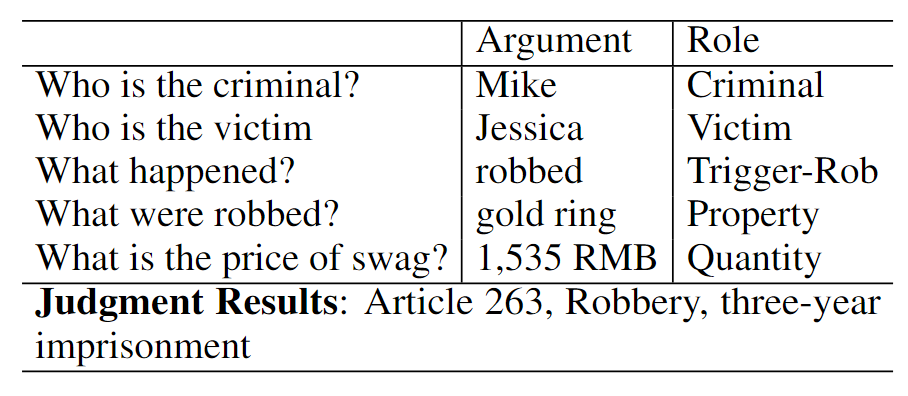
\includegraphics[width=0.6\linewidth]{event.png}
	\caption{事件信息标注样例}
	\label{event}
\end{figure}

\subsubsection{司法证据相关研究现状}

Teng等人针对司法证据研究了司法证据关联相关工作。
刑事案件的司法证据关联将一组司法证据划分为几个不重叠的子集,
提高了司法论点的可解释性和合法性。
证据关联任务是由先前关于法律辅助系统的研究推动的,
特别是提高罪名预测等任务的可解释性。
值得注意的是,划分为相同子集的证据通常用于论证同一个司法论点。
他们提出了一种论证驱动的监督学习方法来计算案件给定证据对之间的距离,
之后根据证据对之间的举例来进行司法证据关联。
除此之外,他们还构建了一个真实的刑事案件证据数据集
进行实验论证结果的有效性。

司法证据的作用是论证用于定罪的若干子论点,
而证据说明是刑事判决书的重要组成部分。
司法判决书中的证据与论点等都是重要的司法元素。
因为在法律判决书中,
法官在撰写判决书时需要立足于事实、证据和法律,
围绕案件的争议焦点、裁判结论和推理过程\upcite{panziqiang}。
如\cref{fig_evidence}所示,
一般刑事判决书中证据部分通常为以下两种表述方法,
左侧利用抽象、笼统的说法或者简单罗列的方法,
代替对证据的分析、论证,
而右侧符合规范的证据说理形式列出了证据与对应分论点的组织结构,
具有更好的可读性,然而此类规范形式在形式判决书中仅占约5\%。

\begin{figure}[h]
	\centering
	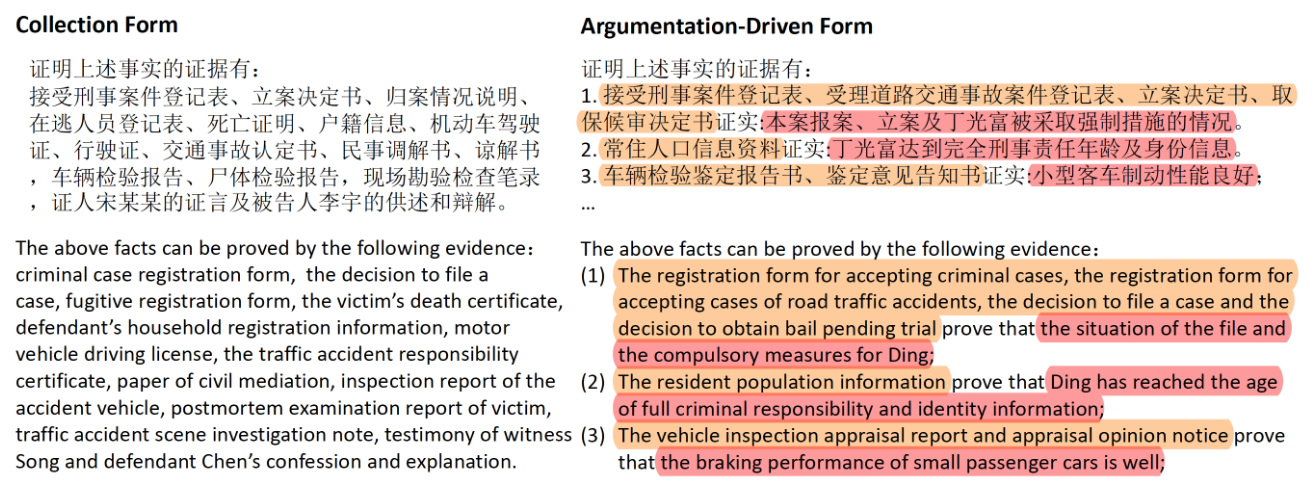
\includegraphics[width=0.9\linewidth]{fig_evidence.png}
	\caption{实际案件中的证据描述的两种形式}
	\label{fig_evidence}
\end{figure}

Teng等人主要使用 BERT\upcite{devlin2018bert}
和 ESIM\upcite{chen2016enhanced} 模型来学习证据对之间的距离度量。
并且发现监督方法能显着提高证据聚类结果。
通过引入来自显式论点的信息,
能够大大提高聚类结果。
但是论文工作存在一定的问题,
因为在大多数实际情况下案件没有给出明确的论点,
所以需要研究如何通过案件描述对判案论点进行建模,
以利用显式判案论点对证据聚类进行改进。

\subsection{研究目标与创新性}
本论文工作拟完成以下几个研究目标:

首先,针对当前司法预测工作
并没有针对案情描述的文本内容与法律条文的维度关联的相关研究的不足,
本工作拟提出一个案情描述文本与法条维度匹配的数据集,
并将在学术界公开。
此外将提出一个案情描述文本重要性预测模型,
实现法律条文与案情描述文本段的对应关系预测。
在此之后,也将基于从案情描述中挖掘的判案论点和抽取的关键信息,
实现一些常见司法预测任务,例如罪名预测等。

其次,针对司法证据预测这个课题现有研究的不足,
本工作拟提出一个司法证据数据集,
并将在学术界公开。
此外将提出一个司法证据预测模型,
实现针对案情描述文本可解释地预测其所需的完备证据集。

最后,将上述的模型组合成完整的司法辅助系统,
开发的软件系统将用于辅助司法从业者以及其他相关人员
分析理解案情信息并做出有关决策。

论文将为智能司法工作,
引入了案情描述文本分析任务和证据预测任务,
提高了其他司法任务的可解释性,
为司法从业者提供了额外的信息来辅助理解和判决案情。

% \textbf{\color{red}(描述论文的目标以及成果,
% 目标是解决什么问题/探索新的方向,成果可以是以下几种形式:
% 1发表论文、2申请专利、3获得软件著作权、4开发装置、5开发软件模块或者系统、6构建一个数据集)}
% 针对XXX领域的不足,研究XXXX方法/开发XXX系统,解决XXX问题或者:
% 探索XXX领域某方面的新思路。研究成果计划发表于XXX会议、申请XXX项发明专利、
% 获得XXX项软件著作权、开发的软件系统将用于XXX、构建的数据集将在学术界公开。
% \textbf{\color{red}(描述论文工作的创新性,与现有研究和工程方案的区别,
% 侧重于理论方法研究的论文可以写方法思路的创新性,侧重于工程实践的论文,
% 可以写系统方案、解决问题的新思路)}
% 论文将引入XXX思路、改进XXX方法、探索XXX理论,从而提高XXX准确率,实现XXX效果、解决XXX问题。
